\documentclass[fleqn]{article}

\usepackage[utf8]{inputenc}
\usepackage[slovak]{babel}
\usepackage[T1]{fontenc}
\usepackage{url}
\usepackage[hidelinks]{hyperref}
\usepackage{graphicx}
\usepackage{caption}
\usepackage{subcaption}
\usepackage{float}
\usepackage{amsmath}
\usepackage{xcolor}
\usepackage{array}
\usepackage{multirow}
\usepackage{units}
\usepackage{unitsdef}
\usepackage[paper=a4paper,margin=1in]{geometry}


\newcommand{\dd}{\text{d}}


\begin{document}
	
\begin{titlepage}
	\begin{center}
		\vspace*{1cm}
		\LARGE
		SLOVENSKÁ TECHNICKÁ UNIVERZITA V BRATISLAVE \\
		\Large
		FAKULTA CHEMICKEJ A POTRAVINÁRSKEJ TECHNOLÓGIE \\
		\vspace*{.5cm}
		\large
		Ústav informatizácie, automatizácie a matematiky \\
		\vspace*{5cm}
		
		\Huge
		\textbf{Modelovanie, dynamika a odhad parametrov biochemických reaktorov}
		
		\vspace{0.5cm}
		\LARGE
		Semestrálna práca
		
		\vspace{1.5cm}
		
		\textbf{Matej Kintler}
		
		\vfill

		\large
		Vedúci práce: doc. Ing. Radoslav Paulen, PhD.
		
		\vspace{1.5cm}
	
		\Large
		Bratislava\\
		13. január 2020
		
	\end{center}
\end{titlepage}

\newgeometry{top=3cm,bottom=3cm,right=3cm,left=3cm}
\newpage

\tableofcontents
\pagestyle{empty}

\newpage
\pagestyle{plain}
\setcounter{page}{1}

\section{Úvod}
Biochemické reaktory sa považujú za dôležitú súčasť chemického priemyslu. Široká škála dôležitých zlúčenín ako farmaceutické produkty, rôzne polyméry alebo produkty potravinárského
% RP: Nemate spell check? Mne to ``potravinárského'' (a nizsie ``kvasiky'', ktore som opravil) podciarkne.
priemyslu sa vyrábajú pomocou určitého fermentačného média (rôzne baktérie, kvasinky, vláknité huby alebo enzýmy) za prísne stanovených podmienok v biochemickom reaktore. Aby sme dokázali zabezpečiť optimálny chod biochemického reaktora z hľadiska ekonomiky, bezpečnosti alebo enviromentálneho zaťaženia, potrebujeme disponovať správnym matematickým modelom, ktorý by adekvátne opisoval správanie daného procesu. Aj keď existuje množstvo matematických modelov, ktoré môžu správne popisovať fungovanie biochemického reaktora, správne identifikovať ich parametre, je často omnoho zložitejšia problematika a je esenciálna pre zabezpečenie optimálnych podmienok.

% RP: Zisiel by sa tu odkaz na literaturu. Prve dve vety si to vyslovene ziadaju.
% RP: Mal by tu byt aj odsek, ktory povie ako je praca koncipovana, t.j. co sa tu clovek dozvie.

\newpage

\section{Biochemický reaktor}
\subsection{Základné informácie}
Biochemický reaktor sa dá vo všeobecnosti definovať ako nádoba, ktorá využíva aktivitu biologického katalyzátora na dosiahnutie požadovanej chemickej premeny.
% RP: Tu je opat celkom vhodne miesto na odkaz na literaturu.
%
Bioreaktor všeobecne poskytuje biomechanické a biochemické prostredie, ktoré riadi prenos živín a kyslíka do buniek a produkty metabolizmu z buniek. Dal by sa tiež označiť ako zariadenie, určené na optimálny rast a metabolickú aktivitu organizmu, pôsobením biokatalyzátora, enzýmu alebo mikroorganizmov a buniek zvierat alebo rastlín. Surovinou môže byť organická alebo anorganická chemická zlúčenina alebo dokonca komplexný materiál. Produkt konverzie môže zahŕňať pekárske kvasinky, proteín, štartovacie kultúry alebo primárne metabolity (napr. aminokyseliny, organické kyseliny, vitamíny, polysacharidy, etanol atď.) a sekundárne metabolity (napr. antibiotiká). Bioreaktory sa môžu použiť na biokonverziu alebo biotransformáciu produktov (steroidná biotransformácia, L-sorbitol), enzýmov (amyláza, lipáza, celuláza), rekombinantných produktov (niektoré vakcíny, hormóny, ako je inzulín a rastové hormóny). Bioreaktor musí byť navrhnutý tak, aby vyhovoval konkrétnemu procesu \cite{ref1}.



\subsection{Typy biochemických reaktorov}
Na základe spôsobu prevádzky môže byť bioreaktor klasifikovaný ako vsádzkový, kontinuálny a polovsádzkový. 
Pri vsádzkovom spôsobe sa sterilné kultivačné médium naočkuje mikroorganizmami. Počas tohto reakčného obdobia sa s časom menia množstvá buniek, substrátu vrátane výživných solí, vitamínov a produktov. Fermentácia prebieha vopred stanovenú dobu a produkt sa zozbiera na konci.
V polovsádzkovom réžime sa do reaktora postupne pridávajú živiny, ako prebiehajú bioreakcie, aby sa získali lepšie výťažky a vyššia selektivita spolu s reguláciou reakčnej teploty. Produkty sa zbierajú na konci výrobného cyklu ako pri vsádzkovom bioreaktore. 
Charakteristickou črtou kontinuálneho bioreaktora je proces neustáleho dodávania substrátu. Prúd kvapaliny alebo suspenzie sa kontinuálne privádza a odstraňuje z reaktora. Na dosiahnutie rovnomerného zloženia a teploty je potrebné mechanické alebo hydraulické miešanie. Kultivačné médium, ktoré je buď sterilné alebo obsahuje mikroorganizmy, sa nepretržite dodáva do bioreaktora, aby sa udržal stabilný stav. Reakčné premenné a kontrolné parametre zostávajú konzistentné a vytvárajú v reaktore časovo konštantný stav. Výsledkom je nepretržitá produktivita.
Tradičné vsádzkové miešacie tankové reaktory (STR) a kontinuálne miešacie tankové
reaktory (CSTR) existujú už po stáročia a sú stále široko prijímané v chemickom a biologickom priemysle kvôli ich jednoduchosti. Ostatné bioreaktory, ktoré majú špeciálne konštrukčné a prevádzkové vlastnosti sú foto-bioreaktory, rotačné bubnové reaktory, hmlový bioreaktor, membránový bioreaktor, bioreaktory s náplňou a fluidnou vrstvou atď. Tieto boli navrhnuté tak, aby vyhovovali špecifickým procesom \cite{ref1}.


\subsection{Parametre opisujúce biochemický reaktor a ich význam}
Hlavné premenné, ktoré opisujú mikrobiálne procesy v prírode sú uvedené v Tabuľke \ref{tab: 1}.

\textit{Množstvo mikroorganizmov} môže byť vyjadrené ako biomasa $(x)$ alebo počet buniek $(N)$ pri jednobunkových organizmoch (baktétrie, kvasinky, spóry) na jednotku pôdy, množstva vody, objemu alebo obsahu plochy. Vláknité organizmy (huby, aktinomycéty) sú charakterizované dĺžkou mycélia $(L)$ a počtom hýf $(n)$. Treba zdôrazniť, že $(n)$ nie je totožné s $(N)$, pretože vetvenie hýf skôr pripomína delenie buniek pri jednobunkových organizmoch. Vzťah medzi $(x)$, $(N)$ a $(L)$ nie je jednoznačný pretože hmota jednotlivých buniek a šírka hýf sa líši v závislosti od organizmu a podmieno rastu. 
% RP: spell check ``podmieno rastu''
Všeobecne možno povedať, že pri nadbytku výživných zlúčenín sa formujú veľké bunky resp. široké hýfy, zatiaľ čo pri hladovaní sa tvoria skôr menšie bunky alebo užšie hýfy. Výber biomasy $(x)$ alebo počet buniek $(N)$ alebo dĺžku mycélia $(L)$ závisí na danom prípade. Biomasa $(x)$ má očividnú výhodu pri skúmaní cyklu uhlíka a živín, zatiaľ čo počet buniek $(N)$ sa preferuje pri skúmaní populácie napr. výskyt mutácií alebo prenos plazmidov \cite{ref2}.

\begin{table}
	\centering
	\caption{Prehľad hlavných dynamických parametrov opisujúcich biochemický reaktor \cite{ref2}.}
	\label{tab: 1}
	\begin{tabular}{p{5cm} p{1.9cm} p{4cm}}
		\hline
		\textbf{Parameter} & \textbf{Symbol} & \textbf{Rozmer} \\ 
		\hline
		Hustota/koncentrácia biomasy & $x$ & \micg bunkovej hmoty na \gram pôdy; \gram bunkovej hmoty \unitfrac{1}{\squaremeter}; \micg bunkovej hmoty na \ml vody\\
		Počet buniek & $N$ & $10^{6}$ buniek na \gram pôdy; $10^{6}$ buniek na \ml vody\\
		Dĺžka mycélia & \liter & \meter na \gram pôdy; \meter na \ml vody\\
		Počet hýf & $n$ & $10^{6}$ na \gram pôdy; $10^{6}$ na \ml vody\\
		Koncentrácia limitujúceho substrátu & $s$ & \milligram na \gram pôdy; \unitfrac{\gram}{\squaremeter};\unitfrac{\gram}{\liter vody}\\
		Koncentrácia produktu & $p$ & \milligram na \gram pôdy; \unitfrac{\gram}{\squaremeter}; \unitfrac{\gram}{\liter} vody\\
		\hline	
	\end{tabular}
\end{table}

\textit{Koncentrácia limitujúceho substrátu} vo vode alebo v pôde, $(s)$, predstavuje množstvo esenciálnej živiny využívanej mikroorganizmami na rast a rozmnožovanie. Bežne nevieme posúdiť všetky potenciálne dostupné živiny a zameriať sa iba na jednu alebo zopár individuálnych zlúčenín alebo triedu
% RP: spell check ``zameriať''
molekúl, ktorá reprezentuje limitujúcu zlúčeninu, pretože chemoorganotrofné mikroorganizmy čerpajú energiu z organických zlúčenín, zatiaľ čo fotosyntetizujúce mikroorganizmy vyžadujú prísun svetla a zdroj fosforum dusíka a železa \cite{ref2}.
% PR: spell check ``fosforum''

\textit{Množstvo produktov} $(p)$. Sem patria všetky medziprodukty a konečné produkty metabolizmu mikroorganizmov, ktoré vznikajú počas rastu. Typickými medziprodultmi sú organické kyseliny vznikajúce počas glykolýzy. Jediný konečný produkt aeróbnej mikrobiálnej dekompozície je oxid uhličitý, avšak pri anaeróbnych podmienkach vznikajú rôzne organické kyseliny, alkoholy, ketóny atď. \cite{ref2}.


\subsection{Matematické modely prietokového biochemického reaktora}
Najjednoduchším matematickým modelom, ktorý opisuje prietokový biochemický reaktor je tzv. Monod model. Tento model je veľmi obľúbený kvôli svojej jednoduchosti. Zakladá sa na dvoch predpokladoch: \text{1)} špecifická rýchlosť rastu buniek závisí od koncentrácie substrátu a  \text{2)} tvorba biomasy je spojená so spotrebou substrátu. Formulácia rovníc, ktoré popisujú materialovú bilanciu biomasy je nasledovná:
% RP: spell check ``materialovú''
\begin{table}[H]
% RP: Nie je to chyba alebo problem, ale tu by prostredie table vobec nemuselo byt a stacil by samotny tabular
	\centering
	\begin{tabular}{ccccc}
		akumulácia & & množstvo & & množstvo \\
		bunkovej & = & vzniknutých & -- & odobraných \\
		hmoty & & buniek & & buniek \\
	\end{tabular}
\end{table}
\noindent a pre materialovú bilanciu substrátu platí:
\begin{table}[H]
	\centering
	\begin{tabular}{ccccccc}
		akumulácia & & množstvo & & množstvo & & množstvo\\
		substrátu & = & dodaného & -- & odobraného & -- & spotrebovaného .\\
		v systéme & & substrátu & & substrátu & & substrátu MO\\
	\end{tabular}
\end{table}
\noindent Ak uvažujeme, že objem reaktora sa nemení a prítok substrátu sa rovná odtoku suspenzie, potom môžme písať: 
\begin{align}
	&V\left(\frac{\dd x}{\dd t}\right) = V\mu(s)x - Fx, \label{eq:1} \\
	&V\left(\frac{\dd s}{\dd t}\right) = Fs_{in} - Fs - V\frac{1}{Y_{x}}\mu(s)x. \label{eq:2}
\end{align}

\noindent Ak obe strany rovníc vydelíme objemom reaktora a označíme si pomer $\frac{F}{V} = D$, rýchlosť riedenia, môžme rovnice \ref{eq:1} a \ref{eq:2} upraviť do nasledovného tvaru:
% RP: Rovnice je lepsie referencovat pomocou \eqref
\begin{align} 
	&\frac{\dd x}{\dd t} = \left(\mu(s) - D\right)x, \text{kde}  \quad \mu(s) = \mu_{m}\frac{s}{K_{M} + s}, \label{eq:3} \\
	&\frac{\dd s}{\dd t} = D\left(s_{in} - s\right) - \frac{1}{Y_{x}}\mu(s)x. \label{eq:4}
\end{align}

\begin{table}
	\centering
	\caption{Parametre Monod modelu, ich symbol a rozmer.}
	\label{tab: 2}
	\begin{tabular}{lll}
		\hline
		\textbf{Parameter} & \textbf{Symbol} & \textbf{Rozmer} \\
		\hline
		Špecifická rýchlosť rastu & $\mu(s)$ & \unitfrac{1}{h} \\
		Maximálna špecifická rýchlosť rastu & $\mu_{m}$ & \unitfrac{1}{h} \\
		Michaelisova konštanta & $K_{M}$ & \unitfrac{g}{L} \\
		Výťažok (biomasa) & $Y_{x}$ & \\
		Objem reaktora & $V$ & \unit{L} \\
		Prietok substrátu/suspenzie & $F$ & \unitfrac{L}{h} \\
		Koncentrácia biomasy & $x$ & \unitfrac{g}{L} \\
		Koncentrácia substrátu & $s$ & \unitfrac{g}{L} \\
		Koncentrácia čerstvého substrátu & $s_{in}$ & \unitfrac{g}{L} \\
		\hline
	\end{tabular}
\end{table}

Rovnice \ref{eq:3} a \ref{eq:4} tvoria najjednoduchší opis biochemického reaktora -- Monod model, a význam jednotlivých parametrov je uvedený v Tabuľke \ref{tab: 2}. Avšak, tento model má množstvo nedostatkov. Nedokáže vysvetliť jednotlivé fázy rastu, ktoré sú pozorované experimentálne a to: lag-fázu, smrť buniek na základe hladovania, tvorbu produktu atď. Tieto nedostatky boli doplnené u tzv. štruktorovaných modelov.
% RP: spell check ``štruktorovaných''

Model, ktorý berie do úvahy aj tvorbu produktu, získame doplnením Monod modelu do nasledovného tvaru:
\begin{align} 
&\frac{\dd x}{\dd t} = \left(\mu(s) - D\right)x, \label{eq:5} \\
&\frac{\dd s}{\dd t} = D\left(s_{in} - s\right) - \frac{1}{Y_{x}}\mu(s)x - \frac{1}{Y_{p}}\nu x, \label{eq:6} \\
&\frac{\dd p}{\dd t} = \nu x - Dp, \label{eq:7}
\end{align}
kde $p$ predstavuje koncentráciu produktu v $gL^{-1}$,
% RP: Tu uz zrazu nie su pouzite units?
$Y_{p}$ je
bezrozmerný
% RP: Po slovensky je ``bezrozmerový''. ``Rozmerný'' znamena majuci velky rozmer.
koefcient
% RP: spell check ``koefcient''
výťažnosti produktu a $\nu$ predstavuje kinetický člen rýchlosti tvorby produktu v jednotkách času napr. $ h^{-1} $. Do rovnice \ref{eq:4} sme doplnili časť, ktorá vraví, že časť substrátu sa spotrebuje na tvorbu produktu a rovnica \ref{eq:7} predstavuje obyčajnú materiálovú bilanciu produktu.

Ak by sme chceli do modelu zakomponovať tendenciu úmrtia mikroorganizmov počas hladovania, treba upraviť špecifickú rýchlosť rastu $\mu(s)$ tak, že bude obsahovať inhibičný člen $ K_i $, ktorého rozmer je $gL^{-1}$.
% RP: S tymto nesuhlasim. Inhibicia modeluje situaciu ked sa prilis vysoka koncentracia substratu stane pre mikroorganizmy toxickou. Dzem musi obsahovat 50% cukru prave preto aby sa nepokazil.
Špecifická rýchlosť rastu potom nadobudne tvar:
\begin{equation} \label{eq:8}
	\mu(s) = \mu_{m}\frac{s}{K_{M} + s + \frac{s^2}{K_i}}.
\end{equation}

\newpage

\section{Analýza matematických modelov}
V predchádzajúcej časti sme spomenuli viacero modelov, ktorými môžeme opísať biochemický reaktor. V tejto časti sa budeme venovať analýze dvoch modelov a to Monod modelu doplnenému o produktovú časť a modelu, taktiež s produktovou časťou, ale s vplyvom inhibície.

\subsection{Dynamika}
Matematický model, ktorý opisuje bioreaktor je nelineárny model. To znamená, že odozva systému je rôzna pre rovnakú veľkosť skokovej zmeny.
% RP: Trocha neuplna veta. ``odozva systému je rôzna pre rovnakú veľkosť skokovej zmeny'' toto je pravda pre rozne pociatocne podmienky a treba to jasne napisat
Túto nelinearitu si možno všimnúť na Obr. \ref{fig:1}.
% RP: Jedna veta nemoze povedat ``pozrite sa na obrazok'' a druha uz predpokladat, ze z obrazka citatel ``najedol''. Obrazok treba popisat. Napr. ``na obrazku je ukazany priebeh vystupu...'' Aka simulacia bola vlastne urobena? Aky model? Ake pociatocne podmienky? Ake vstupy?
Ďalej si môžme všimnúť prudký narást koncentrácie produktu na počiatku, ktorý bol spôsobený nadbytkom biomasy a malým množstvom substrátu v systéme.
% RP: Myslim, ze na ``male mnozstvo substratu'' nema vplyv na produkt. Nakoniec ``s'' sa v rovnici (7) nenachadza.
Po ustálení dynamika produtku pripomímna systém 1. rádu. Na druhej strane v dynamike tvorby biomasy sa prejavuje nestabilná nula (menšie podkmity), ktoré sú spôsobené veľkou časovou konštantou tvorby biomasy a malou časovou konštantou odtoku suspenzie.
% RP; Odtok suspenzie nie je stav, takze nema casovu konstantu. Tento efekt by sa dal vysvetlit krajsie...napisem to len narychlo: v dosledku zvysenie prietoku latky cez reaktor, pritecie viac substratu, cim sa zvysi jeho koncentracia; koncentracia mikroorganizmov sa ale znizi; nasledne zvysena koncentracia substratu podpori rast biomasy a tym sa aj koncetracia biomasy zacne zvysovat.
V dynamike substrátu sa zasa prejavuje stabilná nula, ktorá opäť súvisí s rýchlym prítokom česrstvého média a pomalšou spotrebou na tvorbu biomasy a produktu.
% RP: spell check ``česrstvého''

\begin{figure}
	\centering
	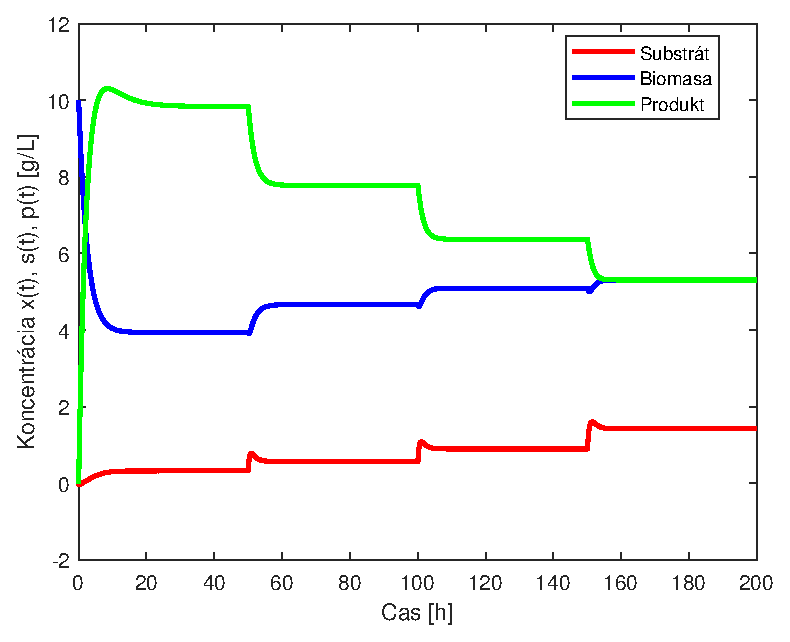
\includegraphics[width=.7\linewidth]{images/step_change}
	\caption[]{Viacnásobná skoková zmena rýchlosti riedenia $D$ pri začiatočných podmienkach $p_0 = s_0 = 0, x_0 = 10 gL^{-1}$.}
	% RP: Popis obrazku musi popisat, co je na obrazku ukazane. Ja tam ``viacnásobnú skokovú zmenu rýchlosti riedenia'' nevidim.
	% RP: Opat su tu ``kurzivove'' jednotky.
	\label{fig:1}
\end{figure}

Režim fungovania bioreaktora má významný vplyv na dynamiku celého systému a pri určitých podmienkach Monod model a model s inhibíciou môžu vykazovať rovnaké správanie, presne ako je tomu na Obr. \ref{fig:1}. Avšak, tieto modely sa odlišujú vo formulácii špecifickej rýchlosti rastu, ktorý má zásadný vplyv na dynamiku systému. Ako vidno na Obr. \ref{fig:2} pri Monod modely
% RP: spell check ``modely''
sa špecifická rýchlosť rastu limitne blíži ku maximálnej špecficikej rýchlosti rastu, zatiaľ čo model s inhibícou dosahuje svoje maximum v bode $S^{*} = \sqrt{K_M K_i}$.
% RP: Nie je jasne co je vlastne ukazane na obrazku. Nikto si len tak ``z prsta nevycuca'' ze ukazujete ustalene stavy. Tie musite predstavit na zaklade modelu.
Pri nesprávne zvolených pracovných podmienkach, či už počiatočných podmienkach systému, koncentrácie čerstvého substrátu alebo rýchlosti riedenia, model s inhibíciou bude vykazovať diametrálne odlišné správanie od Monod modelu, ako to je zobrazené na Obr. \ref{fig:3}.
% RP: Opat treba obrazok popisat. Najlepsia zasada je aby plocha obrazku zodpovedala ploche textu, ktory obrazok opisuje.
% RP: Hodilo by sa tu opisat, co sa deje v tychto dvoch reaktoroch a takisto by sa citatel mal po prvykrat dozvediet, ze existuje nieco ako washout (stav vymytia?) kedy je prevadzka reaktora nenavratne narusena.

\begin{figure}
	\centering
	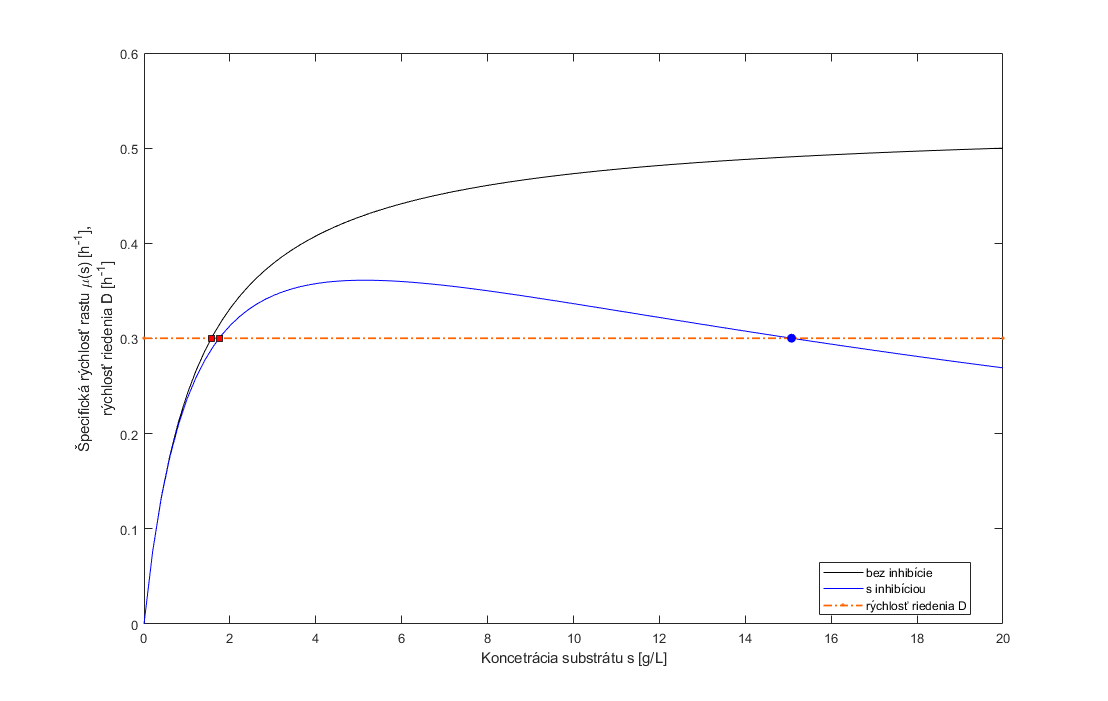
\includegraphics[width=.7\linewidth]{images/spec_grow_rate_comparison}
	\caption[]{Porovnanie priebehu špecifickej rýchlosti rastu Monod modelu (červená) a modelu s inhibíciou (modrá). Červeným štvorčekom sú označené nenulové stabilné ustálené stavy, modrou guličkou je označený nestabilný stav.}
	% RP: Legenda mi pride nekonzistentna. Dal by som odtial prec ``rychlost riedenia D'' a skor uviedol v popise obrazku, ze bodkociarkovanou ciarou je znazornena zvolena rychlost riedenia D = 0.3h^-1
	\label{fig:2}
\end{figure}

\begin{figure}
	\begin{subfigure}{.5\textwidth}
		\centering
		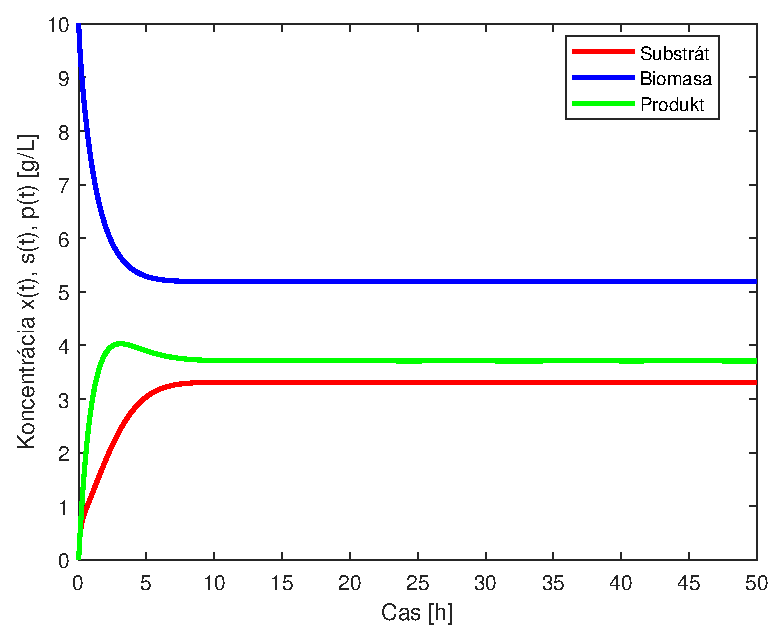
\includegraphics[width=1\linewidth]{images/dyn_Monod}
		\caption[]{Monod model}
	\end{subfigure}
	\begin{subfigure}{.5\textwidth}
		\centering
		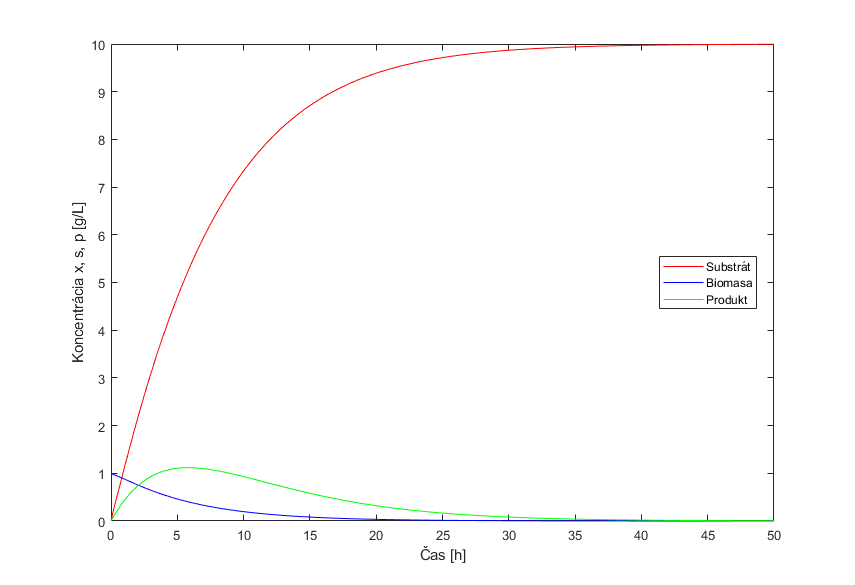
\includegraphics[width=1\linewidth]{images/dyn_inhb}
		\caption[]{Model s inhibíciou}
	\end{subfigure}
	\caption{Porovnanie dynamiky modelov pri rovnakých pracovných podmienkach.}
	\label{fig:3}
\end{figure}


\subsection{Stabilita}
Výhodou prietokových bioreaktorov je, že pri dodržaní správnych podmienok, dokážeme systém uviesť do časovo konštantného stavu, ktorý nepretržito pracuje. Avšak nájdenie správnych parametrov, nemusí byť také triviálne, ako by sa na prvý pohľad mohlo zdať. Z rovnice \ref{eq:5}
vyplýva, že na dosiahnutie ustáleného stavu, je nutné, aby sa špecifická rýchlosť rastu rovnala rýchlosti riedenia, takto získame netriviálne riešenie, alebo je počiatočná koncentrácia biomasy nulová a takto získame triviálne riešenie.
% RP: Nemusi to byt len pociatocna koncentacia biomasy, ktora je nulova. Akonahle x=0 v case T, bude sa x rovnat 0 pre t>T
Na Obr. \ref{fig:2} môžno viďieť nenulové ustálené stavy Monod modelu, ale aj modelu s inhibíciou. Je dobré si všimnúť, že zatiaľ čo Monod model má iba jeden nenulový ustálený stav, model s inhibíciou už obsahuje dva.
% RP: Tento opis musi prist ked uvadzate obrazok a tu sa na existenciu viacerych ustalenych stavovo uz iba odvolavate. 

\begin{figure}
	\begin{subfigure}{.5\textwidth}
		\centering
		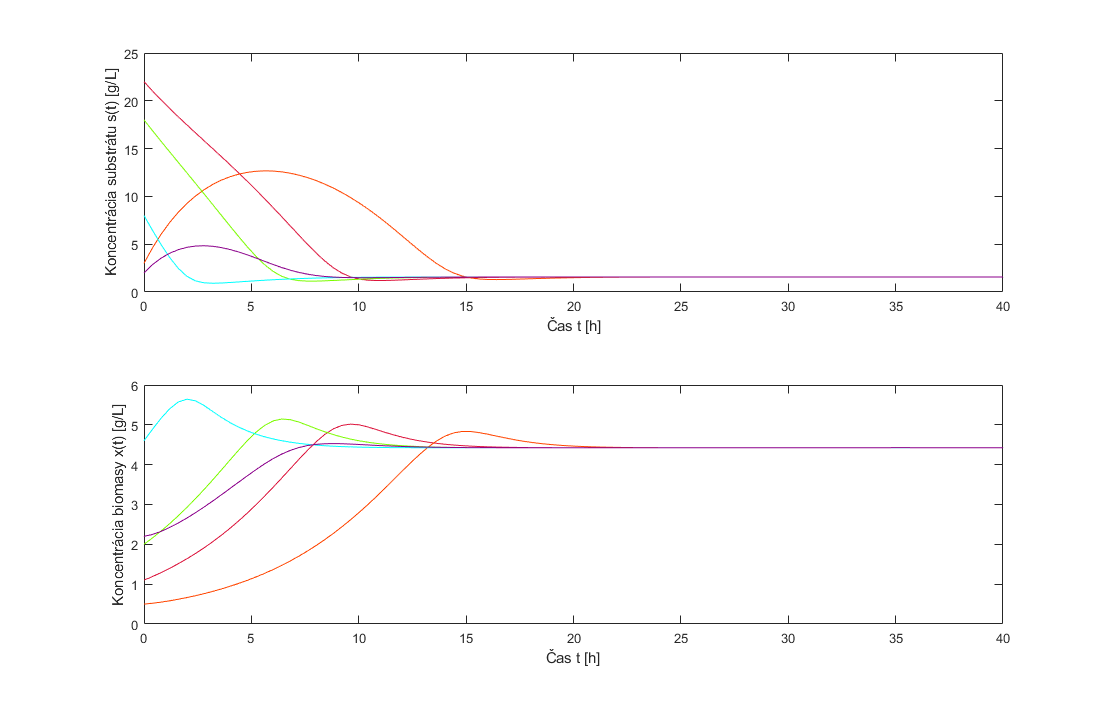
\includegraphics[width=1\linewidth]{images/init_cond_Monod}
		\caption[]{Časový priebeh koncentrácie substrátu a biomasy.}
	\end{subfigure}
	\begin{subfigure}{.5\textwidth}
		\centering
		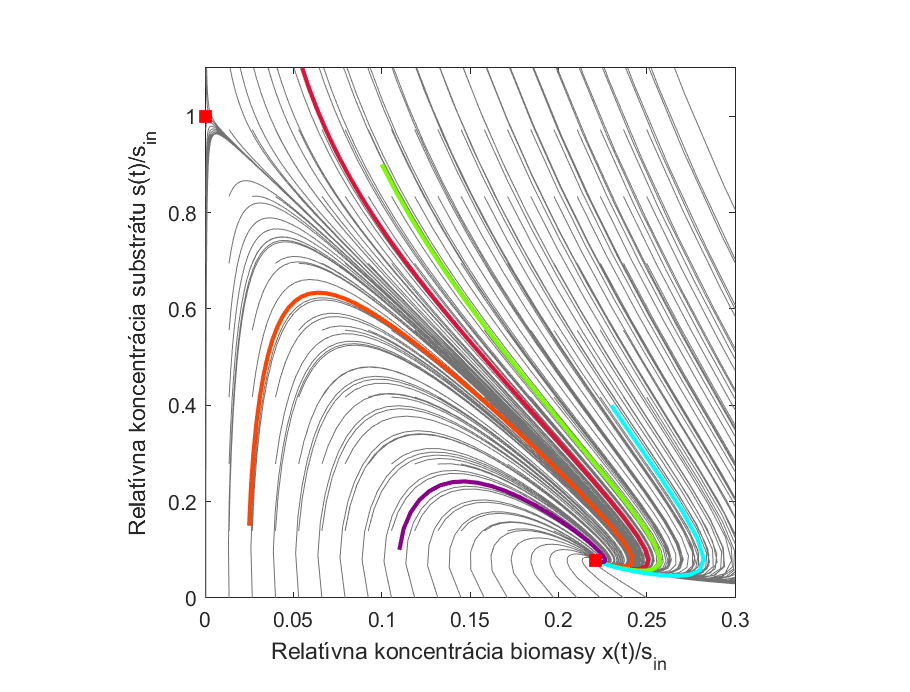
\includegraphics[width=1\linewidth]{images/phase_Monod}
		\caption[]{Fázový diagram.}
	\end{subfigure}
	\caption{Stabilita a ustálený stav Monod modelu pri nastavení parametrov uvedených v Tabuľke \ref{tab: 3}.}
	\label{fig:4}
\end{figure}

Na  fázovom diagrame Monod modelu(Obr. \ref{fig:4} napravo), môžme 
%RP: ``môžme'' nie je po slovensky
vidieť oba ustálené stavy. Ak zvolíme začiatočné podmienky rôzne od nuly (najmä pri koncentrácii biomasy -- vedú k triviálnemu riešeniu a systémom bude pretekať čerstvý substrát) pri konštantnej rýchlosti riedenia menšej alebo rovnej ako špecifická rýchlosť rastu, sa vždy dostaneme do toho istého ustáleného stavu.

Model s inhibíciou vykazuje odlišné správanie. Na fázovom diagrame (Obr.\ref{fig:5} napravo) môžme sledovať už dva nenulové stavy a jeden nulový. Výsledkom triviálneho riešenia je "výplach", ktorý vedie k nulovej koncentrácii biomasy a systémom bude pretekať čerstvý substrát. Ako si môžme všimnúť, vždy keď je rýchlosť rastu biomasy pomaľšia
% RP: spell check ``pomaľšia''
ako je odtok suspenzie zo sýstému, dostneme sa do výplachu.
% RP: Ako som uz pisal vyssie, opis vyplachu musi prist skor. Tu by sa mohlo uz rozobrat aj preco sa do vyplachu system dostane/nedostane

\begin{figure}
	\begin{subfigure}{.5\textwidth}
		\centering
		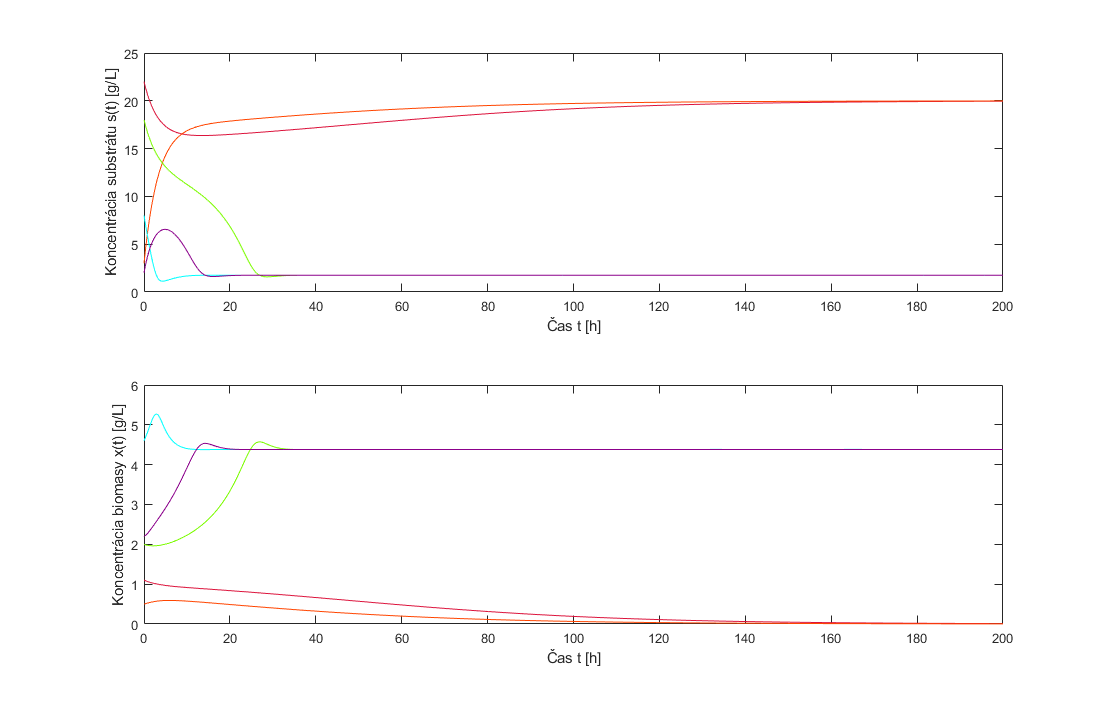
\includegraphics[width=1\linewidth]{images/init_cond_inhb}
		\caption[]{Časový priebeh koncentrácie substrátu a biomasy.}
	\end{subfigure}
	\begin{subfigure}{.5\textwidth}
		\centering
		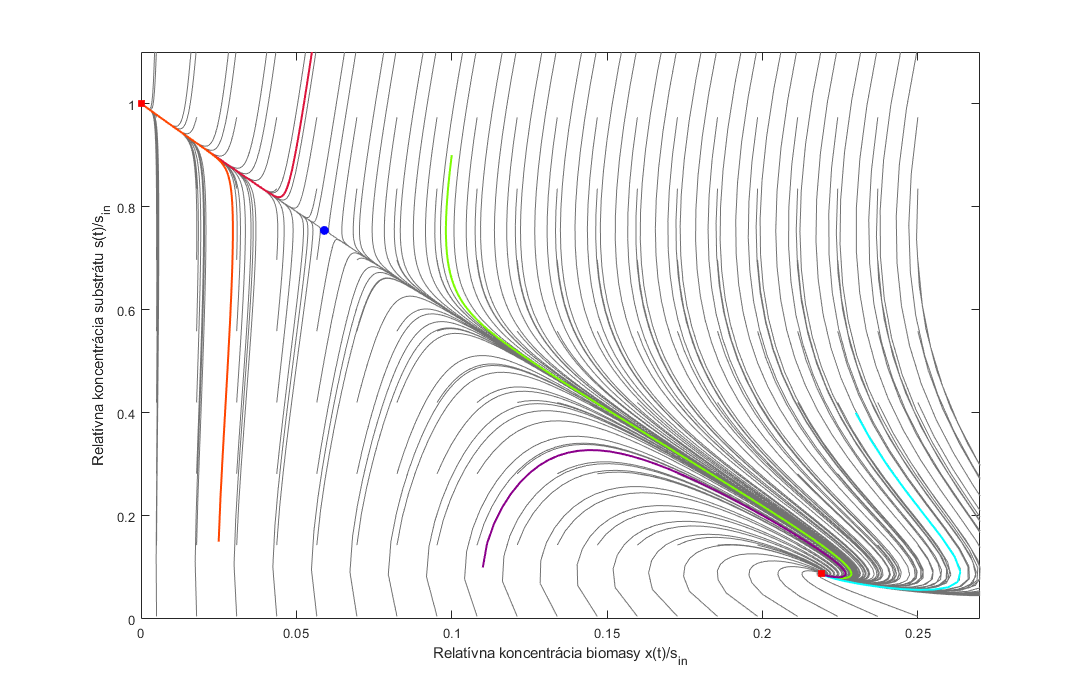
\includegraphics[width=1\linewidth]{images/phase_inhb}
		\caption[]{Fázový diagram. Červeným štvorčekom sú označené stabilné ustálené stavy, modrou guličkou je označený nestabilný stav.}
	\end{subfigure}
	\caption{Stabilita a ustálené stavy modelu s inhibíciou pri nastavení parametrov uvedených v Tabuľke \ref{tab: 3}.}
	\label{fig:5}
\end{figure}

% RP: Nerozumiem takemuto zaciatku odseku ``Ostali ...'' Kde ostali? Novy odsek by mal zacat novu myslienku a zaroven nadviazat na predchadzajuci text.
\noindent Ostali dva netriviálne stavy, z ktorých jeden je nestabilný a druhý je stabilný. V okolí nestabilného stavu môžu nastať dva prípady a to v závislosti od počiatočných podmienok. Ak sa nachádzame na Obr. \ref{fig:2} naľavo, to znamená, že rýchlosť rastu biomasy je väčšia ako odtok suspenzie, dostaneme sa do nenulového ustáleného stavu. Ak sa nachádzame viac napravo, dostaneme sa do výplachu.

\begin{table}
	\centering
	\caption{Nastavenie parametrov Monod modelu a modelu s inhibíciou. Údaje pod čiarou mali danú veľkosť v prípade, že sa nemenili.}
	% RP: Toto je nepresne ``Údaje pod čiarou mali danú veľkosť v prípade, že sa nemenili.'' Nevedel by som na zaklade tohto zopakovat vasu simulaciu. Rozumiem zameru tohto opisu a myslim, ze je dobry ale vysledok je matuci. Dala by sa tu napr. dat vedlajsia tabulka, kde by boli aj stvrty stlpec ``Rozsah'' a tam by sa uviedol rozsah zmien parametrov.
	\label{tab: 3}
	\begin{tabular}{lll}
		\hline
		\textbf{Parameter} & \textbf{Veľkosť} & \textbf{Rozmer} \\
		\hline
	 	$\mu_{m}$ & 0.53 & \unitfrac{1}{\hour} \\
	 	$\nu$ & 0.5 & \unitfrac{1}{\hour} \\
		$K_{M}$ & 1.2 & \unitfrac{\gram}{\liter} \\
		$K_{i}$ & 22 & \unitfrac{\gram}{\liter} \\
		$Y_{x}$ & 0.4 & \\
		$Y_{p}$ & 1 & \\
		$V$ & 3.33 & \liter \\
		$F$ & 1 & \unitfrac{\liter}{\hour} \\
		\hline
		$s_{in}$ & 20 & \unitfrac{\gram}{\liter} \\
		$p_0, s_0$ & 0 & \unitfrac{\gram}{\liter} \\
		$x_0$ & 10 & \unitfrac{\gram}{\liter} \\
		\hline
	\end{tabular}
\end{table}

Ďalší parameter, ktorý dokáže ovplyvniť stabilitu systému, je koncentrácia čerstvého substrátu. Z Obr. \ref{fig:7} je zrejmé, že ak koncentrácia čerstvého roztoku je nižšia ako nejaká minimálna hodnota, náš systém pôjde do výplachu. Koncentrácia čerstvého substrátu ovplyvňuje špecifickú rýchlosť rastu (viď Obr. \ref{fig:2} ). Tým pádom ak sa nachádzame v oblasti pod prvým nenulovým ustáleným stavom (ten v takomto prípade neexistuje, pretože sme mimo pracovného nastavenia) dochádza k výplachu. Ak sa chceme dostať do nenulového ustáleného stavu, je nutné aby koncentrácia čerstvého substrátu bola vyššia ako koncentrácia v prvom nenulovom ustálenom stave.
% RP: Opat rozumiem zameru a je dobry. Vo vysledku ale nerozumiem...najviac ma matu slovne spojenia ``prvy nenulovy''. Podla coho je prvy? Podla coho je nenulovy? Nulovy ustaleny stav by mal (x, s) = (0, 0) a taky nie je.
Pri Monod modely by sme mohli ísť s touto koncentráciou do nekonečna, kde by sme dosiahli maximálnu rýchlosť rastu. Ale na rozdiel od Monod modelu, pri modely s inhibícou, by od istého momentu ($S^{*} = \sqrt{K_M K_i}$) so zväčšujúcou sa koncentráciou čerstvého substrátu klesala špecifická rýchlosť rastu, ktorá sa limitne blíži k nule a koncentrácia biomasy padne na nulu.
% RP: ``padne na nulu'' -> ``klesne na nulu'' je vhodnejsi vyraz

\begin{figure}
	\centering
	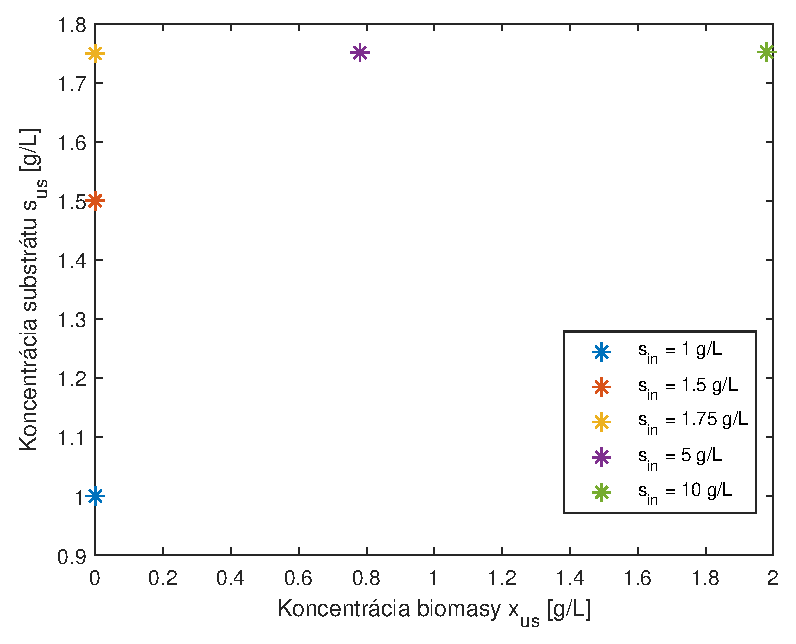
\includegraphics[width=.7\linewidth]{images/s_in_inhb}
	\caption[]{Závislosť koncentrácie substrátu od koncentrácie biomasy v ustálenom stave pri rôznych koncentráciach čerstvého substratu $s_{in}$.}
	\label{fig:7}
\end{figure}

\newpage

\section{Odhad parametrov}
Je zrejmé, že nastaviť optimálny chod biochemického reaktora je zložitá záležitosť a jeho pracovný réžim treba prispôsobiť na základe daného fermentačného média, teda na základe jeho vlastných parametrov -- maximálnej špecifickej rýchlosti rastu, Michaelisovej konštanty a prípadne konštanty inhibície. Tie však nepoznáme a je nutné ich získať z jednotlivých časových priebehov, najčastejšie koncentrácie substrátu.

\subsection{Optimalizačné metódy}
Pri návrhu optimalizácie, by našim cieľom mohlo byť minimalizovať výrobné náklady alebo maximalizovať efektívnosť výroby. Optimalizačný algoritmus je postup, ktorý sa vykonáva iteratívne porovnávaním rôznych riešení, až kým sa nenájde optimálne alebo uspokojivé riešenie. Dnes existujú dva odlišné typy optimalizačných algoritmov.

\begin{itemize}
	\item[\textbf{(a)}] \textbf{Deterministické algoritmy.} 
	Tieto využívajú špecifické pravidlá na posúvanie riešenia od jedného k druhému. Ide o metódy, ktoré sú založené na poznaní gradientu účelovej funkcie alebo na odhade gradientu. Môže sem patriť napr. metóda poklesu gradientu, Newtonova metóda, simplexova (Nelder--Mead) metóda alebo metóda hľadania extrému.
	\item[\textbf{(a)}] \textbf{Stochastické algoritmy.} 
	Tieto majú povahu pravdepodobnostných pravidiel. Stávajú sa veľmi obľúbenými kvôli určitým vlastnostiam, ktoré deterministické algoritmy nemajú. Sem môžu patriť metódy ako simulované žíhanie alebo metóda Luus--Jaakola.
\end{itemize}

Metódy založené na poznaní gradientu účelovej funkcie vedú k lokálnemu optimu, zatiaľ čo stochastické metódy často vedú ku globálnemu optimu, ale vyžadujú značné množstvo vyhodnotení účelovej funkcie. Z tohto dôvodu, pre rozmerovo väčšie problematiky, sú negradientové metódy menej žiadúce.


\subsection{Prístupy k odhadu}
Na začiatku by bolo vhodné spomenúť, že nie vždy dokážeme získať analytické riešenie modelu, ktoré by nám veľmi uľahčilo prácu, pretože by šlo o výrazne jednoduchšiu optimalizačnú úlohu regresie dát. V prípade, že nemáme k dispozícii analytické riešenie, je nutné priebehy modelu počítať numerickými metódami, čo nás privádza k rôznym návrhom optimalizačných problémov. 

Spôsob, akým získať neznáme parametre modelu, môže byť rôzny a zavisí najmä od množstva údajov, ktorými disponujeme. V prípade, že z reálneho zariadenia dokážeme získať viaceré časové priebehy, teda merať, môžeme parametre odhadnúť na základe aproximácie derivácie. Vysvetlíme si to na príklade biochemického reaktora. V prípade, že dokážeme merať časový priebeh koncentrácie biomasy a substrátu, môžeme na základe rovnice \eqref{eq:5} odhadnúť parametre $K_{M}$ a $\mu_{m}$. Optimalizačný problém by mohol byť sformulovaný následovne:

\begin{equation}
	\min_{\mu_{m},K_{M}} \quad \sum_{n=1}^{N} \left(\Delta_{i}^m-\mu(s_i^m,\mu_{m},K_M)\right)^2,  
\end{equation}

\noindent kde $ N $ je celkový počet dát, $ \Delta_{i} = x_{i}^m-x_{i-1}^m $ je diferencia dvoch susedných nameraných hodnôt koncentrácie biomasy, $ s_i^m $ je hodnota nameranej koncentrácie substrátu v \textit{i}--tom bode a tvar špecifickej rýchlosti rastu závisí od daného modelu a môže mať tvar daný buď \eqref{eq:3}, alebo \eqref{eq:8}.

Prvý prístup je síce veľmi jednoduchý, ale má svoje nevýhody. Najväčším problémom je však skutočnosť, že bežne meriame iba koncentráciu substrátu a tým pádom prichádzame o značnú časť informácií. Druhý prístup obchádza tento problém a zameriava sa na hľadanie neznámych parametrov samotných diferenciálnych rovníc. Zatiaľ čo návrh optimalizačného problému sa príliš nezmení, zložitosť výpočtu sa výrazne zvýši. V tomto prípade je nutné, v každom nameranom bode, niekoľkokrát numericky vyhodnotiť priebehy koncentrácie biomasy, produktu a aj substrátu a porovnať ich s nameraným signálom  tak, aby sme získali optimálne riešenie. Túto problematiku by sme mohli sformulovať následovne: 

\begin{equation}
	\begin{aligned}
		\min_{\mu_{m},K_{M}} \quad & \sum_{n=1}^{N} \left(s_{i}^m-s_{i}\right)^2, \\
		\textrm{s.t.} \quad & \dot{s} = D(s_{in}-s)-\frac{1}{Y_x}\mu(s,\mu_{m},K_M)x-\frac{1}{Y_p}\nu x \\
							& \dot{x} = (\mu(s,\mu_{m},K_M)-D)x
	\end{aligned}
\end{equation}

kde $ s_{i} $ je koncentrácia substrátu v \textit{i}--tom bode vypočítaná na základe modelu biochemického reaktora.

Ostáva tu však otázka, ako správne voliť štruktúru špecifickej rýchlosti rastu, aby sme dokázali správne určiť odhadované parametre. Túto informáciu nevieme jednoducho získať z nameraných údajov a môžeme dospieť k nesprávnemu modelu.

\newpage

\section{Výsledky}
V experimentálnej časti sme sa venovali porovaniu prístupov k odhadu parametrov a porovnaniu dvoch optimalizačných metód -- simplexovej (Nelder--Mead) metóde a metóde Luus--Jaakola. Dáta boli vygenerované modelom 
% RP: data boli vygenerovane simulaciou modelu, nie ``vygenerované modelom ''
s inhibíciou pri viacerých skokových zmenách v rýchlosti riedenia $D = $ (0.2, 0.3, 0.4 a 0.5\unitfrac{1}{\hour}) v čase $t = $ 50\unit{\hour} a ich časový priebeh je zobrazený na Obr. \ref{fig:1}. Parametre modelu boli nastavené podobne ako je uvedené v Tabuľke \ref{tab: 3} s rozdielom v maximálnej špecifickej rýchlosti rastu s hodnotou $\mu_{m} = $ 0.954\unitfrac{1}{\hour}. Odhad parametrov sme robili vzhľadom na Monod model, kvôli vyššie uvedeným skutočnostiam. 

Najväčším problémom pri odhade parametrov na základe aproximácie derivácie je šum merania. Diferencia takéhoto signálu vedie k strate údajov z dynamiky systému. Preto je potrebné takýto zašumený signál najskôr spracovať napr. filtráciou. Ďalším faktom je, že meranie koncentrácie biomasy má omnoho väčšiu fluktuáciu ako samotné meranie koncentrácie substrátu, čo vedie k väčším nepresnostiam. V praxi by bolo nutné zabezpečiť identifikáciu živých organizmov od mŕtvych, ak by sme chceli robiť odhad takýmto prístupom. Na Obr. \ref{fig:8} môžeme vidieť výsledok odhadu parametrov na základe aporximácie
% Rp: spell check ``aporximácie''
derivácie. Môžeme si všimnúť, že takýto prístup k odhadu parametrov kladie dôraz skôr na dynamiku systému ako na samotné ustálené stavy.

\begin{figure}
	\centering
	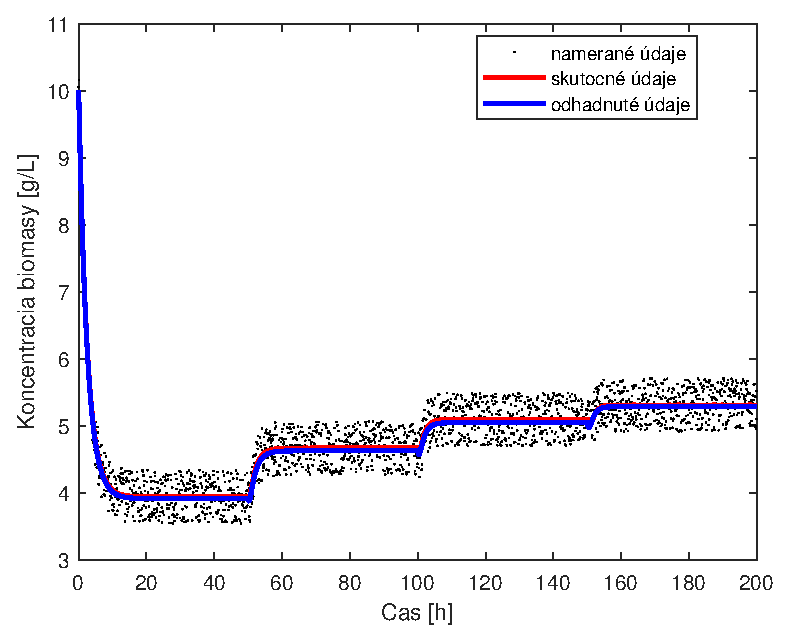
\includegraphics[width=.7\linewidth]{images/der_approximation}
	\caption[]{Časový priebeh koncentrácie biomasy vypočítaný podľa parametrov odhadnutých na základe aproximácie derivácie.}
	\label{fig:8}
\end{figure}

Odhadovať parametre na základe celého modelu je v tomto prípade omnoho efektívnejšie. Vyhneme sa tak spomínaným problémom pri odhade parametrov aproximáciou derivácie. Veľkou výhodou tohto prístupu je, že rozptyl šumu môže byť výrazne väčší. Výsledok takéhoto prístupu k odhadu parametrov môžeme vidieť na Obr. \ref{fig:9}. Z obrázku je očividné, že odhadnutý priebeh je kvalitatívne lepší ako v predchádzajúcom prípade.
% RP: Hm, toto porovnanie nefunguje kedze ste na Obr. 8 neukazali koncentraciu susbstratu. Citatel ma skor pocit, ze ho chcete zavadzat.

\begin{figure}
	\centering
	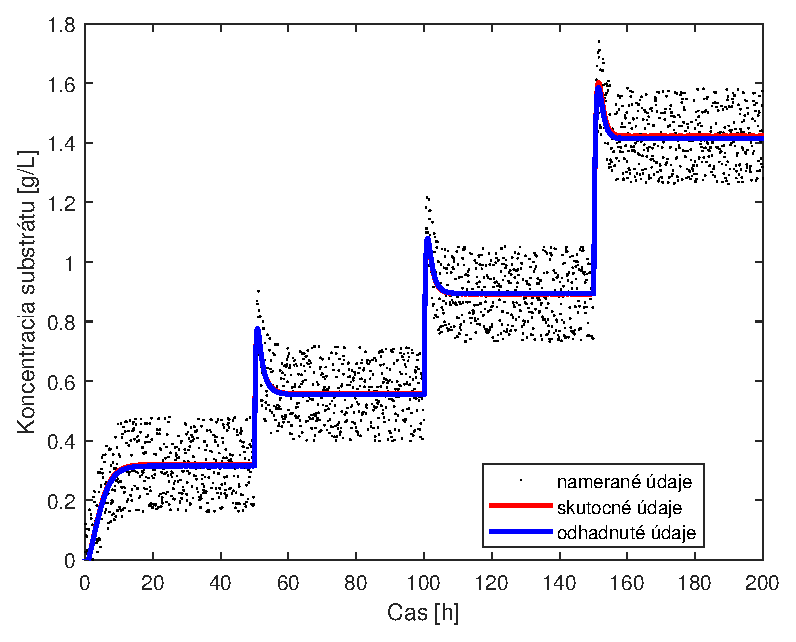
\includegraphics[width=.7\linewidth]{images/param_approx_diff_eq}
	\caption[]{Časový priebeh koncentrácie substrátu vypočítaný podľa parametrov odhadnutých na základe diferenciálnych rovníc modelu a nameranej koncentrácie substrátu.}
	\label{fig:9}
\end{figure}

Výsledky porovnania optimalizačných metód pri odhade parametrov na základe modelu a nameranej koncentrácie substrátu sú uvedené v Tabuľke \ref{tab: 4}. Simplexová metóda bola v každom bode efektívnejšia ako metóda Luus--Jaakola. Rozdiel pri týchto metódach je ten, že zatiaľ čo metóda Luus--Jaakola je čisto stochastická metóda, ktorá náhodne umiestňuje body, v ktorých vyhodnocuje účelovú funkciu a porovnáva ju z predchádzajúcimi bodmi, simplexová metóda funguje na aproximácií gradientu a pohybuje sa teda tou najrýchlejšou možnou cestou.
% RP: Simplexova metoda gradient priamo neaproximuje. Dalo by sa skor povedat nieco ako, ze svoj dalsi postup voli na zaklade predoslych hodnot ucelovej funckie. Najrychlejsia mozna by zrejme bola Newtonova metoda, ale ta by si vyzadovali vypocitanie (to nie je uplne jednoduche) alebo aproximaciu gradientu a dokonca aj Hessianu.
Ako už bolo spomínané, tento prístup k odhadu je výpočtovo veľmi náročný, keďže je nutné numericky vyhodnocovať priebeh modelu v každom bode. Tým pádom každé jedno vyhodnotenie účelovej funkcie zaberie značné množstvo času. Ani jedna z týchto metód však nevedie ku globálnemu optimu, ale sú založené na tolerancii nepresnosti.
% RP: V skutocnosti sa aj globalne optimum da najst iba s nejakou odchylkou. ``tolerancia nepresnosti'' je zvlastny vyraz.
Z tohto dôvodu by sme dokázali odhadnúť parametre modelu presnejšie, ak by sme znížili toleranciu nepresnosti.

\begin{table}
	\centering
	\caption{Porovnanie optimalizačných metód pri odhade parametrov modelu biochemického reaktora. Skutočné hodnoty boli: maximálna špecifická rýchlosť rastu $\mu_{m} = $ 0.954 \unitfrac{1}{\hour} a Michaelisova konštanta $K_{M} = $ 1.2 \unitfrac{\gram}{\liter}.}
	\label{tab: 4}
	\begin{tabular}{lll}
		\hline
		& \textbf{Nelder--Mead} & \textbf{Luus--Jaakola} \\
		\hline
		$\mu_{m}$ [\unitfrac{1}{\hour}] & 0.8772 & 1.0500 \\
		$K_{M}$ [\unitfrac{\gram}{\liter}] & 1.0667 & 1.5082 \\
		Počet iterácií & 52 & 349 \\
		Počet vyhodnotení účelovej funkcie & 99 & 698 \\
		Čas [\second] & 4.0351 & 75.0524 \\
		\hline
	\end{tabular}
\end{table}

Zvyšné nepresnosti
% RP: Ake nepresnosti? Ved ten model celkom sedi?
boli spôsobené voľbou nesprávnej štruktúry nášho odhadovaného modelu.
% RP: Volbu nespravnej struktury treba opisat lepsie. Teraz to znie ako by ste niekde urobili chybu. Mali by ste popisat, ze cielom Vasho simulacneho experimentu je ako dopadne odhad parametrov ak by sme zvolili nevhodnu strukturu modelu. Na pocudovanie to dopadne velmi dobre a toto je samozrejme dost rizikove lebo ak model strukturne nesedi (napr. by tam boli nejake skryte/nenajdene nuly) tak sa lahko stane, ze navrhnuty regulator alebo optimalizator setpointu privedie reaktor do stavu vymytia
Žiaľ, tieto informácie nedokážeme získať z nameraných údajov a treba tento problém vyriešiť iným spôsobom. Ako bolo ukázané v článku \cite{HERNANDEZ201946}, jedným z riešení môžu byť hybridné modely. Hybridné modely sú také modely, ktoré majú základ v mechanických modeloch a tieto sú doplnené dátovými modelmi. Dátové modely v tomto prípade úpravujú odchýlky od skutočného modelu, ktoré sa iteratívne aktualizujú na základe informácii zo zariadenia (skutočného modelu). Základnou myšlienkou je vynútiť prispôsobenie podmienok optimality medzi zariadením a rozšíreným modelom pomocou podmienok lineárnej korekcie.

\newpage

\section{Záver}
Táto práca sa zaoberala problematikou modelov prietokového biochemického reaktora. Na začiatku sme ozrejmili, čo vlastne biochemický reaktor je, aké funkcie plní a vysvetlili sme rozdiely medzi jednotlivými typmi. Odvodili sme najjednoduchší model biochemického reaktora, tzv. Monod model, ktorý sme následne doplnili o časť tvorby produktu. Následne sme sa zaoberali rozdielmi v dynamike a stabilite Monod modelu a modelu s inhibíciou, ktoré boli ilustrované pomocou fázových diagramov. Najväčšiu časť našej pozornosti sme však venovali odhadu parametrov modelu biochemického reaktora. Tu sme porovnávali rôzne prístupy k odhadu parametrov a jednotilivé optimalizačné metódy. Z výsledkov môžeme tvrdiť, že zatiaľ čo odhad parametrov pomocou aproximácie derivácie vykazoval mnohé nedostatky (napr. citlivosť na šum merania, musíme mať k dispozícií časový priebeh koncentrácie substrátu a aj biomasy, s čím súvisia ďalšie problémy atď.), odhad parametrov na základe diferenciálnych rovníc ich odstránil. Avšak náročnosť na výpočet sa tým výrazne zvýšila. Z optimalizačných metód sa ako najvhodnejšia javila simplexová metóda (viď Tabuľku \ref{tab: 4}). Táto dokázala optimalizačný problém vyriešiť efektívnejšie v porovnaní s metódou Luus--Jaakola. Na samotný záver sme uviedli problematiku štruktúry modelu, kde vhodným riešením tohto problému sa javia byť tzv. hybridné modely. 
\newpage

\bibliographystyle{plain}
\bibliography{literatura}

\end{document}